\documentclass{article}\usepackage[]{graphicx}\usepackage[]{color}
%% maxwidth is the original width if it is less than linewidth
%% otherwise use linewidth (to make sure the graphics do not exceed the margin)
\makeatletter
\def\maxwidth{ %
  \ifdim\Gin@nat@width>\linewidth
    \linewidth
  \else
    \Gin@nat@width
  \fi
}
\makeatother

\definecolor{fgcolor}{rgb}{0.345, 0.345, 0.345}
\newcommand{\hlnum}[1]{\textcolor[rgb]{0.686,0.059,0.569}{#1}}%
\newcommand{\hlstr}[1]{\textcolor[rgb]{0.192,0.494,0.8}{#1}}%
\newcommand{\hlcom}[1]{\textcolor[rgb]{0.678,0.584,0.686}{\textit{#1}}}%
\newcommand{\hlopt}[1]{\textcolor[rgb]{0,0,0}{#1}}%
\newcommand{\hlstd}[1]{\textcolor[rgb]{0.345,0.345,0.345}{#1}}%
\newcommand{\hlkwa}[1]{\textcolor[rgb]{0.161,0.373,0.58}{\textbf{#1}}}%
\newcommand{\hlkwb}[1]{\textcolor[rgb]{0.69,0.353,0.396}{#1}}%
\newcommand{\hlkwc}[1]{\textcolor[rgb]{0.333,0.667,0.333}{#1}}%
\newcommand{\hlkwd}[1]{\textcolor[rgb]{0.737,0.353,0.396}{\textbf{#1}}}%
\let\hlipl\hlkwb

\usepackage{framed}
\makeatletter
\newenvironment{kframe}{%
 \def\at@end@of@kframe{}%
 \ifinner\ifhmode%
  \def\at@end@of@kframe{\end{minipage}}%
  \begin{minipage}{\columnwidth}%
 \fi\fi%
 \def\FrameCommand##1{\hskip\@totalleftmargin \hskip-\fboxsep
 \colorbox{shadecolor}{##1}\hskip-\fboxsep
     % There is no \\@totalrightmargin, so:
     \hskip-\linewidth \hskip-\@totalleftmargin \hskip\columnwidth}%
 \MakeFramed {\advance\hsize-\width
   \@totalleftmargin\z@ \linewidth\hsize
   \@setminipage}}%
 {\par\unskip\endMakeFramed%
 \at@end@of@kframe}
\makeatother

\definecolor{shadecolor}{rgb}{.97, .97, .97}
\definecolor{messagecolor}{rgb}{0, 0, 0}
\definecolor{warningcolor}{rgb}{1, 0, 1}
\definecolor{errorcolor}{rgb}{1, 0, 0}
\newenvironment{knitrout}{}{} % an empty environment to be redefined in TeX

\usepackage{alltt}
\usepackage{amscd, amssymb, amsmath, verbatim, setspace}
\usepackage[left=1.0in, right=1.0in, top=1.0in, bottom=1.0in]{geometry}
\usepackage{mathrsfs}
\usepackage{listings}


\IfFileExists{upquote.sty}{\usepackage{upquote}}{}
\begin{document}
\begin{flushright}
Arif Ali\\
Math 611 Stochastic Simulation\\
Nov 17, 2016\\
\end{flushright}

\begin{center}
\LARGE\textbf{Homework 11}
  \end{center}
\section*{Exercise 1}
\subsection*{Gibbs Sampler from Example 7.2}
From Example 7.2 in the book, we are given the conditional distribution
\begin{equation}
\theta|x \sim Beta(x+a,n-x+b)
\end{equation}
By the properties of the beta distribution:
\begin{equation}
E[\theta|x]=\frac{x+a}{x+a+n-x+b}=\frac{x+a}{a+n+b}
\end{equation}
\begin{knitrout}
\definecolor{shadecolor}{rgb}{0.969, 0.969, 0.969}\color{fgcolor}\begin{kframe}
\begin{alltt}
\hlcom{## code from Example 7.2}
\hlcom{## note: rb is the Rao-Blackwellization vectors I created to calculate}
\hlstd{Nsim}\hlkwb{=}\hlnum{5000}
\hlstd{n}\hlkwb{=}\hlnum{15}
\hlstd{a}\hlkwb{=}\hlnum{3}
\hlstd{b}\hlkwb{=}\hlnum{7}
\hlstd{X}\hlkwb{=}\hlstd{t}\hlkwb{=}\hlstd{rb}\hlkwb{=}\hlkwd{array}\hlstd{(}\hlnum{0}\hlstd{,}\hlkwc{dim}\hlstd{=}\hlkwd{c}\hlstd{(Nsim,}\hlnum{1}\hlstd{))}
\hlstd{t[}\hlnum{1}\hlstd{]}\hlkwb{=}\hlkwd{rbeta}\hlstd{(}\hlnum{1}\hlstd{,a,b)}
\hlstd{X[}\hlnum{1}\hlstd{]}\hlkwb{=}\hlkwd{rbinom}\hlstd{(}\hlnum{1}\hlstd{,n,t[}\hlnum{1}\hlstd{])}
 \hlkwa{for} \hlstd{(i} \hlkwa{in} \hlnum{2}\hlopt{:}\hlstd{Nsim)\{}
  \hlcom{#rb[i-1] = 1/(i-1)*sum((X+a))/(a+n+b)}
  \hlstd{X[i]}\hlkwb{=}\hlkwd{rbinom}\hlstd{(}\hlnum{1}\hlstd{,n,t[i}\hlopt{-}\hlnum{1}\hlstd{])}
  \hlstd{t[i]}\hlkwb{=}\hlkwd{rbeta}\hlstd{(}\hlnum{1}\hlstd{,a}\hlopt{+}\hlstd{X[i],n}\hlopt{-}\hlstd{X[i]}\hlopt{+}\hlstd{b)}
 \hlstd{\}}
  \hlstd{rb} \hlkwb{=} \hlkwd{cumsum}\hlstd{((X}\hlopt{+}\hlstd{a)}\hlopt{/}\hlstd{(a}\hlopt{+}\hlstd{n}\hlopt{+}\hlstd{b))}\hlopt{/}\hlstd{(}\hlnum{1}\hlopt{:}\hlstd{Nsim)}

\hlkwd{plot}\hlstd{((}\hlkwd{cumsum}\hlstd{(t)}\hlopt{/}\hlstd{(}\hlnum{1}\hlopt{:}\hlstd{Nsim)),}\hlkwc{type}\hlstd{=}\hlstr{"l"}\hlstd{)}
\hlkwd{lines}\hlstd{(rb,}\hlkwc{col}\hlstd{=}\hlstr{"red"}\hlstd{)}
\end{alltt}
\end{kframe}
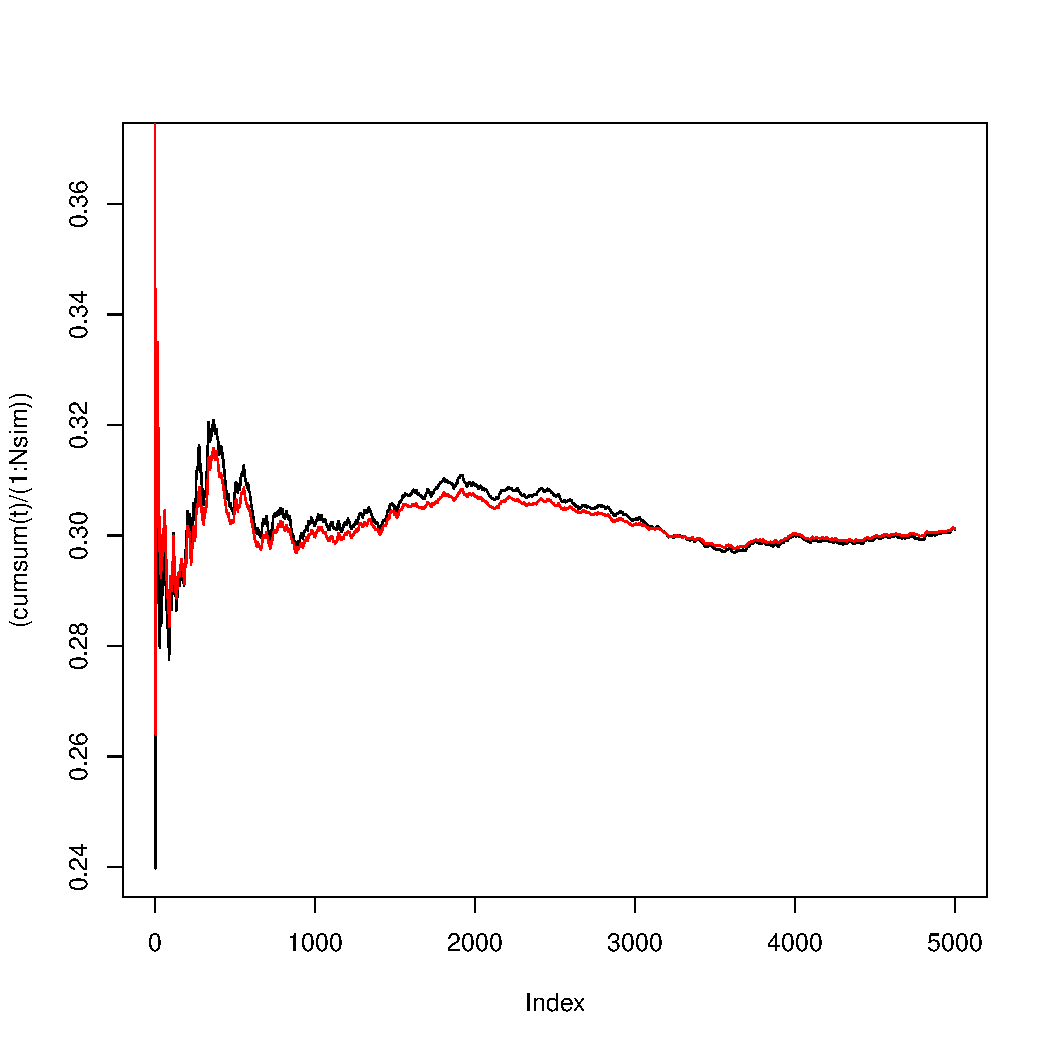
\includegraphics[width=0.60\linewidth]{figure/unnamed-chunk-2-1} 

\end{knitrout}
\section*{Exercise 2}
\subsection*{Part A}
please notes that:
\begin{equation}
f(y|p) = f(y|p,\theta)
\end{equation}
By Bayes rule the following is true:
\begin{equation}
\begin{split}
f(y|p,\theta) \propto f(p,y,\theta) = f(\theta)*f(p|\theta)*f(y|p,\theta) = \\
\frac{1}{a}*e^{-\frac{\theta}{a}}*\theta*p^{\theta-1}*\left(\begin{array}{c}
n\\
y
\end{array}\right)*p^{y}*(1-p)^{n-y} \propto \\
p^{\theta-1}*p^{y}*(1-p)^{n-y} = \\
p^{\theta+y-1}*(1-p)^{(n-y+1)-1} \propto \\
\frac{1}{\beta(\theta+y,n-y+1)}*p^{\theta+y-1}*(1-p)^{(n-y+1)-1} \sim beta(\theta+y,n-y+1))
\end{split}
\end{equation}

\subsection*{Part B}
\begin{equation}
\begin{split}
f(\theta| y,p) \propto f(p,y,\theta) \propto e^{-\frac{a}{\theta}}*\theta*p^{\theta-1}  \propto\\
\theta^{2-1}*e^{-\frac{\theta}{a}}*p^{\theta} = \\
\theta^{2-1}*e^{-\frac{\theta}{a}}*e^{log(p^{\theta})} = \\
\theta^{2-1}*e^{-\frac{\theta}{a}}*e^{(\theta)*log(p)} = \\
\theta^{2-1}*e^{-\frac{\theta}{a}+(\theta)*log(p)} = \\
\theta^{2-1}*e^{-(\frac{1}{a}-log(p))*\theta} = \\
\theta^{2-1}*e^{-\frac{\theta}{(\frac{1}{a}-log(p))^{-1}}} \propto X
\end{split}
\end{equation}

\begin{equation}
X \sim Gamma(2, (\frac{1}{a}+*log(p))^{-1})
\end{equation}

\subsection*{Part C}
\begin{knitrout}
\definecolor{shadecolor}{rgb}{0.969, 0.969, 0.969}\color{fgcolor}\begin{kframe}
\begin{alltt}
\hlstd{a} \hlkwb{=} \hlnum{1}
\hlstd{p} \hlkwb{=} \hlnum{0.5}
\hlstd{n} \hlkwb{=} \hlnum{10}
\hlstd{theta} \hlkwb{=} \hlkwd{rgamma}\hlstd{(}\hlnum{1}\hlstd{, a)}
\hlstd{y} \hlkwb{=} \hlkwd{rbinom}\hlstd{(}\hlnum{1}\hlstd{,n,p)}
\hlstd{Nsim} \hlkwb{=} \hlnum{5e3}
 \hlkwa{for} \hlstd{(i} \hlkwa{in} \hlnum{2}\hlopt{:}\hlstd{Nsim)\{}
  \hlstd{theta[i]} \hlkwb{=} \hlkwd{rgamma}\hlstd{(}\hlnum{1}\hlstd{,} \hlnum{2}\hlstd{,} \hlkwc{scale} \hlstd{= (}\hlnum{1}\hlopt{/}\hlstd{a}\hlopt{-}\hlkwd{log}\hlstd{(p[i}\hlopt{-}\hlnum{1}\hlstd{]))}\hlopt{^-}\hlnum{1}\hlstd{)}
  \hlstd{y[i]} \hlkwb{=} \hlkwd{rbinom}\hlstd{(}\hlnum{1}\hlstd{, n, p[i}\hlopt{-}\hlnum{1}\hlstd{])}
  \hlstd{p[i]} \hlkwb{=} \hlkwd{rbeta}\hlstd{(}\hlnum{1}\hlstd{, y[i]}\hlopt{+}\hlstd{theta[i],n}\hlopt{-}\hlstd{y[i]}\hlopt{+}\hlnum{1}\hlstd{)}

 \hlstd{\}}
\hlkwd{plot}\hlstd{(p, theta)}
\end{alltt}
\end{kframe}
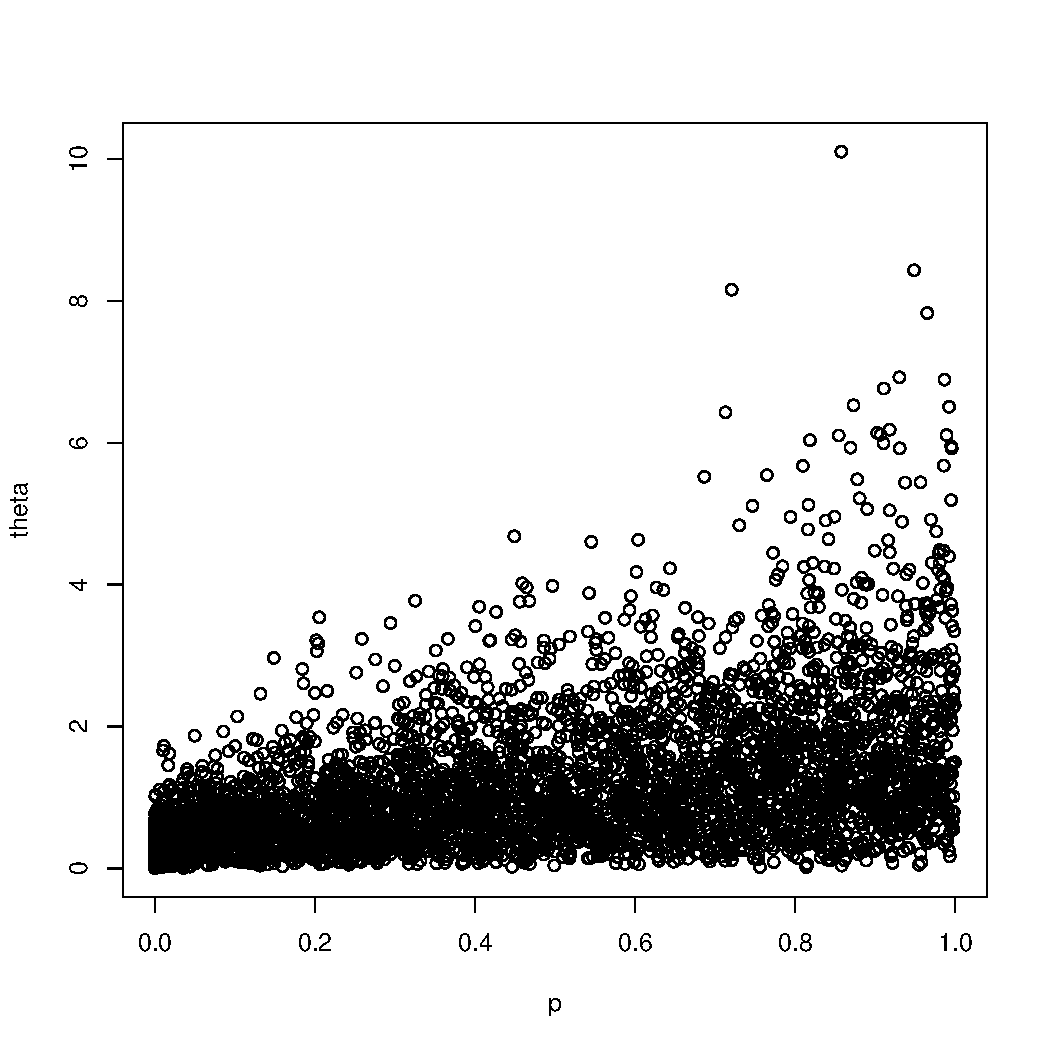
\includegraphics[width=0.60\linewidth]{figure/unnamed-chunk-3-1} 
\begin{kframe}\begin{alltt}
\hlkwd{plot}\hlstd{(}\hlkwd{density}\hlstd{(p))}
\end{alltt}
\end{kframe}
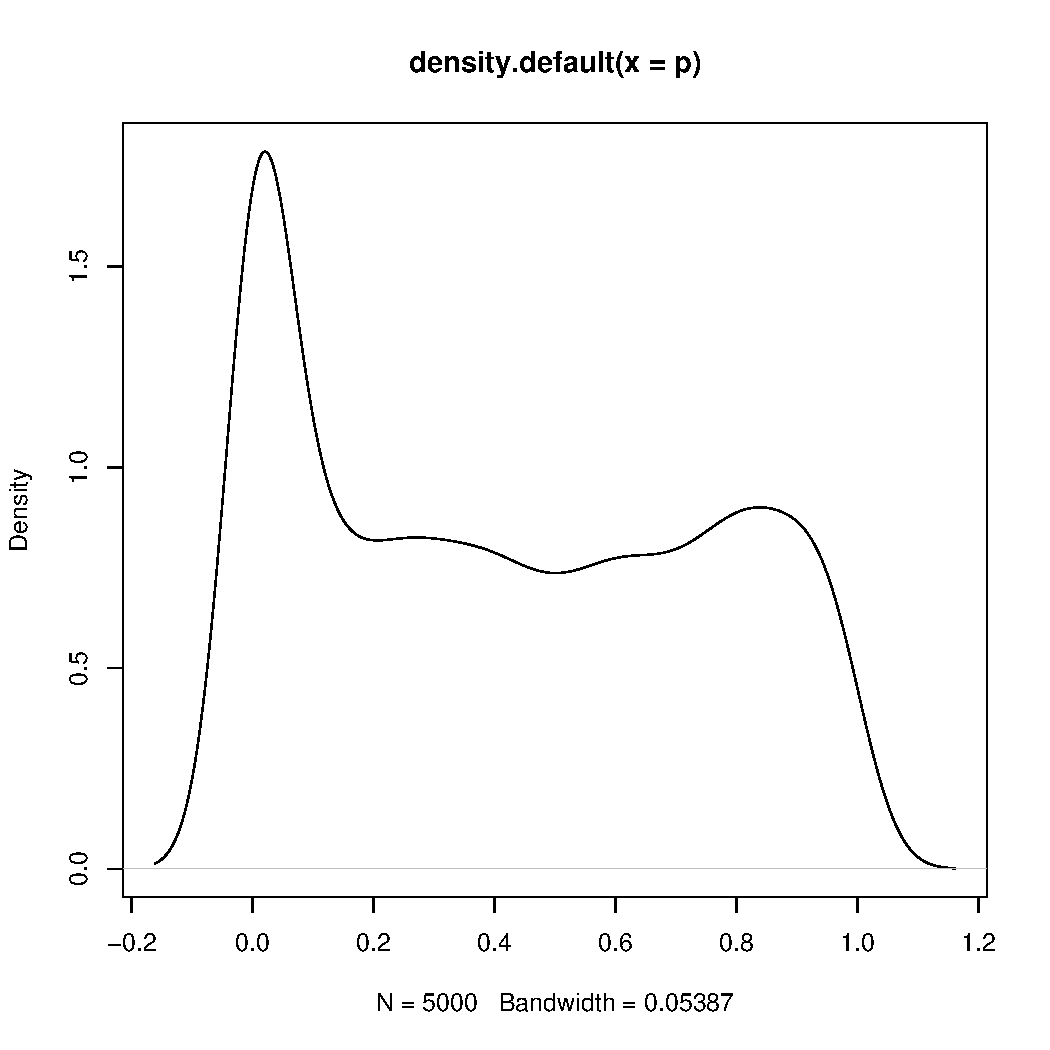
\includegraphics[width=0.60\linewidth]{figure/unnamed-chunk-3-2} 

\end{knitrout}

\section*{Exercise 3}
Note that $gamma(1,\beta)=exponential(\beta)$

\begin{equation}
\begin{split}
\int_{0}^{y} \beta*e^{-\beta*x}dx=0.5 = \\
1-e^{-\beta*y} = 0.5 \implies \\
-exp(-\beta*y) = -0.5 \implies \\
exp(-\beta*y) = 0.5 \implies \\
-\beta*y = ln(0.5) \implies \\
-\beta*y = -ln(2) \implies \\
y = \frac{ln(2)}{\beta}
\end{split}
\end{equation}
Using bcanon we obtain the following:
\begin{knitrout}
\definecolor{shadecolor}{rgb}{0.969, 0.969, 0.969}\color{fgcolor}\begin{kframe}
\begin{alltt}
\hlstd{median_expo} \hlkwb{=} \hlkwa{function}\hlstd{(}\hlkwc{beta}\hlstd{)\{}\hlkwd{log}\hlstd{(}\hlnum{2}\hlstd{)}\hlopt{/}\hlstd{beta\}}
\hlkwd{library}\hlstd{(bootstrap)}
\hlstd{bootstrap_exponential} \hlkwb{=} \hlkwa{function}\hlstd{(}\hlkwc{x}\hlstd{,} \hlkwc{beta}\hlstd{,} \hlkwc{N} \hlstd{=} \hlnum{1e4}\hlstd{,} \hlkwc{alpha_int} \hlstd{=} \hlkwd{c}\hlstd{(}\hlnum{0.05}\hlstd{,} \hlnum{0.95}\hlstd{))\{}
  \hlstd{aa} \hlkwb{=} \hlkwd{bcanon}\hlstd{(x, N,} \hlkwc{theta} \hlstd{= median,} \hlkwc{alpha} \hlstd{= alpha_int)}
\hlstd{\}}
\hlstd{x} \hlkwb{=} \hlkwd{rexp}\hlstd{(}\hlnum{1e4}\hlstd{,} \hlkwc{rate} \hlstd{=} \hlnum{2}\hlstd{)}
\hlstd{bs_medians} \hlkwb{=} \hlkwd{bootstrap_exponential}\hlstd{(x,} \hlnum{2}\hlstd{)}
\hlstd{bs_medians}\hlopt{$}\hlstd{confpoints[}\hlnum{1}\hlstd{,}\hlnum{2}\hlstd{]}\hlopt{<}\hlkwd{median_expo}\hlstd{(}\hlnum{2}\hlstd{)}
\end{alltt}
\begin{verbatim}
## bca point 
##      TRUE
\end{verbatim}
\begin{alltt}
\hlstd{bs_medians}\hlopt{$}\hlstd{confpoints[}\hlnum{2}\hlstd{,}\hlnum{2}\hlstd{]}\hlopt{>}\hlkwd{median_expo}\hlstd{(}\hlnum{2}\hlstd{)}
\end{alltt}
\begin{verbatim}
## bca point 
##      TRUE
\end{verbatim}
\end{kframe}
\end{knitrout}
The median of $gamma(1,\beta)$ is 0.3465736, which is within the 90\% BCa confidence Interval of (0.3399802,0.3567573).

Instead of using a function from the the R package, we adapt the R function build in class.
\begin{knitrout}
\definecolor{shadecolor}{rgb}{0.969, 0.969, 0.969}\color{fgcolor}\begin{kframe}
\begin{alltt}
\hlstd{boot.BCa} \hlkwb{<-}
  \hlkwa{function}\hlstd{(}\hlkwc{x}\hlstd{,} \hlkwc{th0}\hlstd{,} \hlkwc{th}\hlstd{,} \hlkwc{Stat}\hlstd{,} \hlkwc{conf} \hlstd{=} \hlnum{.90}\hlstd{) \{}
    \hlcom{# BCa confidence interval}
    \hlcom{# th0: observed statistic}
    \hlcom{# th: vector of bootstrap distribution}
    \hlcom{# stat is the function to compute the statistic}

    \hlstd{x} \hlkwb{<-} \hlkwd{as.matrix}\hlstd{(x)}
    \hlstd{n} \hlkwb{<-} \hlkwd{nrow}\hlstd{(x)} \hlcom{#observations in rows}
    \hlstd{N} \hlkwb{<-} \hlnum{1}\hlopt{:}\hlstd{n}
    \hlstd{alpha} \hlkwb{<-} \hlstd{(}\hlnum{1} \hlopt{+} \hlkwd{c}\hlstd{(}\hlopt{-}\hlstd{conf, conf))}\hlopt{/}\hlnum{2}
    \hlstd{zalpha} \hlkwb{<-} \hlkwd{qnorm}\hlstd{(alpha)}

    \hlcom{# the bias correction factor}
    \hlstd{z0} \hlkwb{<-} \hlkwd{qnorm}\hlstd{(}\hlkwd{sum}\hlstd{(th} \hlopt{<} \hlstd{th0)} \hlopt{/} \hlkwd{length}\hlstd{(th))}

    \hlcom{# the acceleration factor (jackknife est.)}
    \hlstd{th.jack} \hlkwb{<-} \hlkwd{numeric}\hlstd{(n)}
    \hlkwa{for} \hlstd{(i} \hlkwa{in} \hlnum{1}\hlopt{:}\hlstd{n) \{}
      \hlstd{th.jack[i]} \hlkwb{<-} \hlkwd{Stat}\hlstd{(x[}\hlopt{-}\hlstd{i, ])} \hlcom{#unlike the class example, we are calculating the median of a function }
    \hlstd{\}}
    \hlstd{L} \hlkwb{<-} \hlkwd{mean}\hlstd{(th.jack)} \hlopt{-} \hlstd{th.jack}
    \hlstd{a} \hlkwb{<-} \hlkwd{sum}\hlstd{(L}\hlopt{^}\hlnum{3}\hlstd{)}\hlopt{/}\hlstd{(}\hlnum{6} \hlopt{*} \hlkwd{sum}\hlstd{(L}\hlopt{^}\hlnum{2}\hlstd{)}\hlopt{^}\hlnum{1.5}\hlstd{)}

    \hlcom{# BCa conf. limits}
    \hlstd{adj.alpha} \hlkwb{<-} \hlkwd{pnorm}\hlstd{(z0} \hlopt{+} \hlstd{(z0}\hlopt{+}\hlstd{zalpha)}\hlopt{/}\hlstd{(}\hlnum{1}\hlopt{-}\hlstd{a}\hlopt{*}\hlstd{(z0}\hlopt{+}\hlstd{zalpha)))}
    \hlstd{limits} \hlkwb{<-} \hlkwd{quantile}\hlstd{(th, adj.alpha,} \hlkwc{type}\hlstd{=}\hlnum{6}\hlstd{)}
    \hlkwd{list}\hlstd{(}\hlstr{"est"}\hlstd{=th0,} \hlstr{"BCa"}\hlstd{=limits)}
  \hlstd{\}}
\hlstd{x} \hlkwb{=} \hlkwd{rexp}\hlstd{(}\hlnum{1e4}\hlstd{,} \hlkwc{rate} \hlstd{=} \hlnum{2}\hlstd{)}
\hlstd{boot.median} \hlkwb{=} \hlkwd{c}\hlstd{()}
\hlkwa{for}\hlstd{(i} \hlkwa{in} \hlnum{1}\hlopt{:}\hlnum{1e4}\hlstd{)\{}
  \hlstd{boot.median[i]} \hlkwb{=} \hlkwd{median}\hlstd{(}\hlkwd{sample}\hlstd{(x,} \hlkwc{size} \hlstd{=} \hlnum{1e4}\hlstd{,} \hlkwc{replace} \hlstd{= T))}
  \hlstd{\}}

\hlstd{bca_int} \hlkwb{=} \hlkwd{boot.BCa}\hlstd{(}\hlkwc{x} \hlstd{=} \hlkwd{rexp}\hlstd{(}\hlnum{1e4}\hlstd{,} \hlkwc{rate} \hlstd{=} \hlnum{2}\hlstd{),} \hlkwc{th0} \hlstd{=} \hlkwd{median}\hlstd{(x),} \hlkwc{th} \hlstd{= boot.median ,}\hlkwc{Stat} \hlstd{= median)}\hlopt{$}\hlstd{BCa}
\hlstd{bca_int[}\hlnum{1}\hlstd{]}\hlopt{<}\hlkwd{median_expo}\hlstd{(}\hlnum{2}\hlstd{)}
\end{alltt}
\begin{verbatim}
## 4.736841% 
##      TRUE
\end{verbatim}
\begin{alltt}
\hlstd{bca_int[}\hlnum{2}\hlstd{]}\hlopt{>}\hlkwd{median_expo}\hlstd{(}\hlnum{2}\hlstd{)}
\end{alltt}
\begin{verbatim}
## 94.72531% 
##      TRUE
\end{verbatim}
\end{kframe}
\end{knitrout}
The median of $gamma(1,\beta)$ is 0.3465736, which is within the 90\% BCa confidence Interval of (0.3429105,0.3589501).

If instead of BCa confidence intervals we did Percentile Confidence Intervals, that 90\% Confidence interval would be (0.3431754,0.3589769).
\end{document}
